% Prof. Dr. Ausberto S. Castro Vera
% UENF - CCT - LCMAT - Curso de Ci\^{e}ncia da Computa\c{c}\~{a}o
% Campos, RJ,  2023
% Disciplina: Paradigmas de Linguagens de Programa\c{c}\~{a}o
% Aluno: Mariana Cossetti Dalfior

%%%*****************************************************************************************%%%
\chapter{Aspectos Avan\c{c}ados da Linguagem Python}
%%%*****************************************************************************************%%%
Neste cap\'{\i}tulo ser\~{a}o apresentados os aspectos avan\c{c}ados da linguagem de programa\c{c}\~{a}o Python, incluindo classes, dados de cole\c{c}\~{a}o e fun\c{c}\~{o}es geradoras.

%%%=========================================================================================%%%
\section{Classes}
%%%=========================================================================================%%%
De acordo com \cite{Ramalho2022} Python oferece algumas maneiras de construir uma classe simples que \'{e} apenas uma cole\c{c}\~{a}o de campos, com pouca ou nenhuma funcionalidade extra. Esse padr\~{a}o \'{e} conhecido como \textquotedblleft{}classe de dados\textquotedblright{} \textemdash{} e as classes de dados s\~{a}o um dos pacotes que suportam esse padr\~{a}o.

%%%.........................................................................................%%%		
	\subsection{Classes base Abstratas}
%%%.........................................................................................%%%
As classes abstratas podem ser utilizadas do m\'{o}dulo \textsl{collections.abc} como \textsl{Mapping} e \textsl{MutableMapping}. Idealmente, uma fun\c{c}\~{a}o deve aceitar argumentos desses tipos abstratos e n\~{a}o tipos concretos. Isso d\'{a} mais flexibilidade ao chamador. Considere esta assinatura de fun\c{c}\~{a}o:

\begin{lstlisting}
>>> # Usar abc.Mapping permite que o chamador forneca uma 
>>> # instancia de dict, defaultdict, ChainMap, uma subclasse 
>>> # UserDict ou qualquer outro tipo que seja um subtipo 
>>> # de Mapping.
>>>
>>> from collections.abc import Mapping
>>> def nome2hex(nome: str, color_map: Mapeamento[str, int]) -> str:
\end{lstlisting}

%%%=========================================================================================%%%
\section{Tipos de Dados de Cole\c{c}\~{a}o}
%%%=========================================================================================%%%
Os tipos de dados de cole\c{c}\~{a}o s\~{a}o utilizados para guardar cole\c{c}\~{o}es de valores de acordo com \cite{Perkovic2016}. Esses podem ser divididos em dois: tipos sequenciais e tipos conjuntos.
%%%.........................................................................................%%%
\subsection{Tipos Sequenciais}
%%%.........................................................................................%%%
Os tipos sequenciais s\~{a}o utilizados para armazenar dados em sequ\^{e}ncia, ou seja, em uma ordem espec\'{\i}fica. Existem tr\^{e}s tipos de sequ\^{e}ncia em Python, as listas, tuplas e strings (exibido anteriormente nesse cap\'{\i}tulo em \ref{subsec:str}):				

%%%¨¨¨¨¨¨¨¨¨¨¨¨¨¨¨¨¨¨¨¨¨¨¨¨¨¨¨¨¨¨¨¨¨¨¨¨¨¨¨¨¨¨¨¨¨¨¨¨¨¨¨¨¨¨¨¨¨¨¨¨¨¨¨¨¨¨¨¨¨¨¨¨¨¨¨¨¨¨¨¨¨¨¨¨¨¨¨¨¨%%%
\subsubsection{Listas} \label{cap3/3.2.1}
%%%¨¨¨¨¨¨¨¨¨¨¨¨¨¨¨¨¨¨¨¨¨¨¨¨¨¨¨¨¨¨¨¨¨¨¨¨¨¨¨¨¨¨¨¨¨¨¨¨¨¨¨¨¨¨¨¨¨¨¨¨¨¨¨¨¨¨¨¨¨¨¨¨¨¨¨¨¨¨¨¨¨¨¨¨¨¨¨¨¨%%%
As listas s\~{a}o cole\c{c}\~{o}es ordenadas de elementos que podem ser de diferentes tipos de dados - como inteiros, strings, booleanos e at\'{e} outras listas. Elas s\~{a}o uma das estruturas mais utilizadas em Python por serem muito vers\'{a}teis - podendo ser modificadas removendo, alterando e adicionando novos elementos ap\'{o}s a sua cria\c{c}\~{a}o. As listas s\~{a}o criadas utilizando \textsl{'[]'} e seus elementos s\~{a}o separados por v\'{\i}rgulas e indexados de forma num\'{e}rica - inicia com \'{\i}ndice 0 para o primeiro elemento e vai aumentando de um em um para os \'{\i}ndices posteriores. A seguir \'{e} poss\'{\i}vel observar o c\'{o}digo fonte \ref{fontelistas1} e o resultado \ref{resullistas1} do exemplo da utiliza\c{c}\~{a}o de listas em Python:

\begin{lstlisting}
>>> # utilizando apenas numeros inteiros
>>> num = [1, 2, 3, 4, 5]
>>> print(num[4])
5

>>> # utilizando apenas strings 
>>> vasco = ["Andrey", "Puma", "Pedro Raul"]
>>> print(vasco[1])
Puma

>>> # utilizando de forma mista
>>> junto = [7, "Piton", 5.0, False]
>>> print(junto[3])
False
\end{lstlisting}

\begin{figure}[H]
	\begin{center}
		\caption{C\'{o}digo fonte do exemplo do uso listas} \label{fontelistas1}
		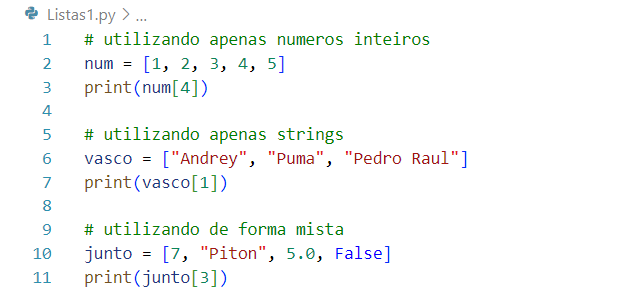
\includegraphics[width=12cm]{listas1} 
		\newline
		Fonte: Criado por Mariana Cossetti Dalfior
	\end{center}
\end{figure}

\begin{figure}[H]
	\begin{center}
		\caption{Resultado do c\'{o}digo fonte do exemplo do uso listas} \label{resullistas1}
		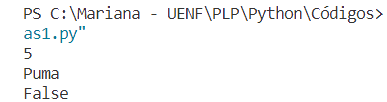
\includegraphics[width=9cm]{resullistas1} 
		\newline
		Fonte: Criado por Mariana Cossetti Dalfior
	\end{center}
\end{figure}

\'{E} poss\'{\i}vel realizar opera\c{c}\~{o}es comuns nas listas utilizando os m\'{e}todos, como \textsl{'.append()'}, \textsl{'.extend()'}, \textsl{'.insert()'}, \textsl{'.remove()'}, \textsl{'.pop()'}, \textsl{'.index()'}, \textsl{'.count()'} e \textsl{'.sort()'}. A seguir \'{e} poss\'{\i}vel observar o c\'{o}digo fonte \ref{fontelistas2} e o resultado \ref{resullistas2} do exemplo da utiliza\c{c}\~{a}o de m\'{e}todos em listas:

\begin{lstlisting}
>>> # utilizando append
>>> num = [1, 2, 3, 4, 5]
>>> num.append(6)
>>> print(num)
[1, 2, 3, 4, 5, 6]

>>> # utilizando extend 
>>> num = [2, 4, 6]
>>> impares = [1, 3, 5]
>>> num.extend(impares)
>>> print(num)
[1, 2, 3, 4, 5, 6]

>>> # utilizando insert
>>> num = [1, 2, 3, 4, 5]
>>> num.insert(1, 'Vasco')
>>> print(num)
[1, 'Vasco', 2, 3, 4, 5]
	
\end{lstlisting}

\begin{figure}[H]
	\begin{center}
		\caption{C\'{o}digo fonte do exemplo da utiliza\c{c}\~{a}o de m\'{e}todos em listas} \label{fontelistas2}
		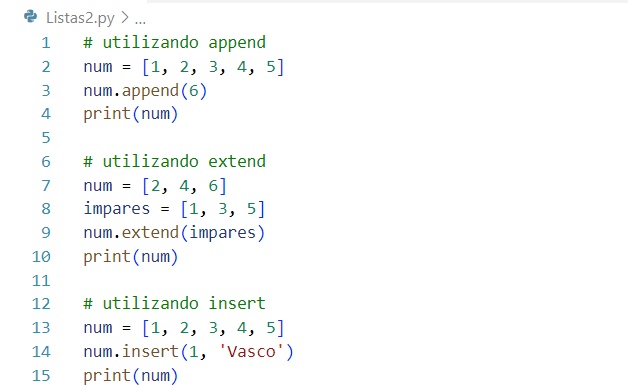
\includegraphics[width=12cm]{listas2} 
		\newline
		Fonte: Criado por Mariana Cossetti Dalfior
	\end{center}
\end{figure}

\begin{figure}[H]
	\begin{center}
		\caption{Resultado do c\'{o}digo fonte do exemplo da utiliza\c{c}\~{a}o de m\'{e}todos em listas} \label{resullistas2}
		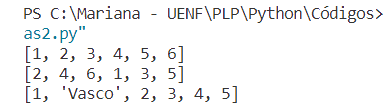
\includegraphics[width=9cm]{resullistas2} 
		\newline
		Fonte: Criado por Mariana Cossetti Dalfior
	\end{center}
\end{figure}

%%%¨¨¨¨¨¨¨¨¨¨¨¨¨¨¨¨¨¨¨¨¨¨¨¨¨¨¨¨¨¨¨¨¨¨¨¨¨¨¨¨¨¨¨¨¨¨¨¨¨¨¨¨¨¨¨¨¨¨¨¨¨¨¨¨¨¨¨¨¨¨¨¨¨¨¨¨¨¨¨¨¨¨¨¨¨¨¨¨¨%%%
\subsubsection{Tuplas}
%%%¨¨¨¨¨¨¨¨¨¨¨¨¨¨¨¨¨¨¨¨¨¨¨¨¨¨¨¨¨¨¨¨¨¨¨¨¨¨¨¨¨¨¨¨¨¨¨¨¨¨¨¨¨¨¨¨¨¨¨¨¨¨¨¨¨¨¨¨¨¨¨¨¨¨¨¨¨¨¨¨¨¨¨¨¨¨¨¨¨%%%
As tuplas s\~{a}o um tipo de dado de cole\c{c}\~{a}o, parecidos com as listas, diferente delas possui como caracter\'{\i}sticas serem imut\'{a}veis - n\~{a}o podem ser modificadas depois de sua cria\c{c}\~{a}o. Al\'{e}m disso, elas geralmente s\~{a}o usadas para o armazenamento de dados que s\~{a}o relacionados, diferente das listas que s\~{a}o utilizadas para armazenar cole\c{c}\~{o}es de objetos. As tuplas s\~{a}o criadas de diversas maneiras em Python, por\'{e}m a mais comum \'{e} utilizando par\^{e}nteses \textsl{'()'}. Exemplo da utiliza\c{c}\~{a}o de tuplas em Python: 

\begin{lstlisting}
>>> # criando tupla de valor inteiro
>>> tupla1 = (1, 2, 3, 4, 5)

>>> # criando tupla de string
>>> tupla2 = ('a', 'b', 'c', 'd', 'e')

>>> # criando tupla de booleano
>>> tupla3 = (True, False, True, True)
\end{lstlisting}	

Uma tupla pode conter diferentes tipos de dados, como n\'{u}meros, strings e booleanos. As tuplas tamb\'{e}m podem ser indexadas e fatiadas da mesma maneira que as listas. No entanto, como as tuplas s\~{a}o imut\'{a}veis, n\~{a}o \'{e} poss\'{\i}vel alterar um elemento individual da tupla depois que ela foi criada.	
%%%.........................................................................................%%%
\subsection{Tipos Conjunto}
%%%.........................................................................................%%%
Na linguagem Python existem dois tipos de conjuntos: o set e o frozenset.
%%%¨¨¨¨¨¨¨¨¨¨¨¨¨¨¨¨¨¨¨¨¨¨¨¨¨¨¨¨¨¨¨¨¨¨¨¨¨¨¨¨¨¨¨¨¨¨¨¨¨¨¨¨¨¨¨¨¨¨¨¨¨¨¨¨¨¨¨¨¨¨¨¨¨¨¨¨¨¨¨¨¨¨¨¨¨¨¨¨¨%%%
\subsubsection{Set}
%%%¨¨¨¨¨¨¨¨¨¨¨¨¨¨¨¨¨¨¨¨¨¨¨¨¨¨¨¨¨¨¨¨¨¨¨¨¨¨¨¨¨¨¨¨¨¨¨¨¨¨¨¨¨¨¨¨¨¨¨¨¨¨¨¨¨¨¨¨¨¨¨¨¨¨¨¨¨¨¨¨¨¨¨¨¨¨¨¨¨%%%
O set \'{e} uma cole\c{c}\~{a}o de elementos \'{u}nicos e mut\'{a}veis criados usando chaves \textsl{'\{\}'} ou a fun\c{c}\~{a}o \textsl{'set()'}, onde a ordem dos elementos n\~{a}o \'{e} garantida. O conjunto pode ser de diferentes tipos de dados - como inteiros, strings e outras cole\c{c}\~{o}es. Ademais, \'{e} poss\'{\i}vel fazer opera\c{c}\~{o}es matem\'{a}ticas entre conjuntos - como uni\~{a}o, interse\c{c}\~{a}o e diferen\c{c}a. A seguir \'{e} poss\'{\i}vel observar o c\'{o}digo fonte \ref{fonteset} e o resultado \ref{resulset} do exemplo da utiliza\c{c}\~{a}o do set em Python:
\begin{lstlisting}
>>> # Criando um conjunto
>>> conjunto1 = {1, 2, 3, 4, 5}
>>> print(conjunto1)  
{1, 2, 3, 4, 5}

>>> # Criando um conjunto vazio
>>> conjunto2 = set()
>>> print(conjunto2)  
set()

>>> # Removendo um elemento do conjunto
>>> conjunto1.remove(3)
>>> print(conjunto1) 
{1, 2, 4, 5}

>>> # Adicionando um elemento ao conjunto
>>> conjunto1.add(6)
>>> print(conjunto1) 
{1, 2, 3, 4, 5, 6}

>>> # Operacoes entre conjuntos
>>> conjunto2 = {4, 5, 6, 7, 8}
>>> print(conjunto1.union(conjunto2)) 
{1, 2, 3, 4, 5, 6, 7, 8}
>>> print(conjunto1.intersection(conjunto2)) 
{4, 5}
>>> print(conjunto1.difference(conjunto2)) 
{1, 2, 3}
\end{lstlisting}	

\begin{figure}[H]
	\begin{center}
		\caption{C\'{o}digo fonte do exemplo do uso do \textsl{set}} \label{fonteset}
		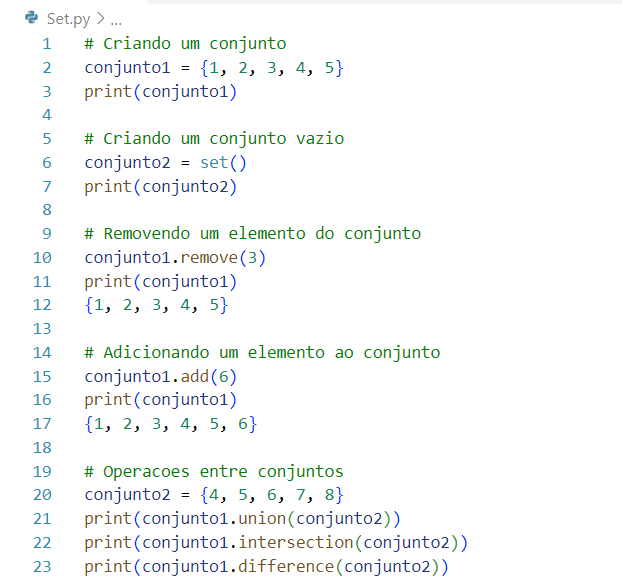
\includegraphics[width=12cm]{set} 
		\newline
		Fonte: Criado por Mariana Cossetti Dalfior
	\end{center}
\end{figure}

\begin{figure}[H]
	\begin{center}
		\caption{Resultado do c\'{o}digo fonte do exemplo do uso do \textsl{set}} \label{resulset}
		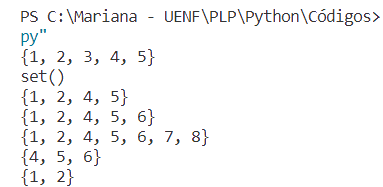
\includegraphics[width=9cm]{resulset} 
		\newline
		Fonte: Criado por Mariana Cossetti Dalfior
	\end{center}
\end{figure}

%%%¨¨¨¨¨¨¨¨¨¨¨¨¨¨¨¨¨¨¨¨¨¨¨¨¨¨¨¨¨¨¨¨¨¨¨¨¨¨¨¨¨¨¨¨¨¨¨¨¨¨¨¨¨¨¨¨¨¨¨¨¨¨¨¨¨¨¨¨¨¨¨¨¨¨¨¨¨¨¨¨¨¨¨¨¨¨¨¨¨%%%
\subsubsection{Frozenset}
%%%¨¨¨¨¨¨¨¨¨¨¨¨¨¨¨¨¨¨¨¨¨¨¨¨¨¨¨¨¨¨¨¨¨¨¨¨¨¨¨¨¨¨¨¨¨¨¨¨¨¨¨¨¨¨¨¨¨¨¨¨¨¨¨¨¨¨¨¨¨¨¨¨¨¨¨¨¨¨¨¨¨¨¨¨¨¨¨¨¨%%%
O frozenset \'{e} uma cole\c{c}\~{a}o de elementos \'{u}nicos e imut\'{a}veis criados usando a fun\c{c}\~{a}o \textsl{'frozenset()'}, por\'{e}m a ordem desses elementos n\~{a}o \'{e} garantida. O conjunto imut\'{a}vel pode ser de diferentes tipos de dados - como inteiros, strings e outras cole\c{c}\~{o}es. Contudo, n\~{a}o possibilita a adi\c{c}\~{a}o, remo\c{c}\~{a}o ou mudan\c{c}a de elementos ap\'{o}s a cria\c{c}\~{a}o. A seguir \'{e} poss\'{\i}vel observar o c\'{o}digo fonte \ref{fontefrozenset} e o resultado \ref{resulfrozenset} do exemplo da utiliza\c{c}\~{a}o do frozenset em Python: \newline

\begin{lstlisting}
>>> # Criando um conjunto imutavel
>>> num = frozenset([2, 4, 6, 8, 10])
>>> print(num)
frozenset({2, 4, 6, 8, 10})
\end{lstlisting}	

\begin{figure}[H]
	\begin{center}
		\caption{C\'{o}digo fonte do exemplo do uso do \textsl{frozenset}} \label{fontefrozenset}
		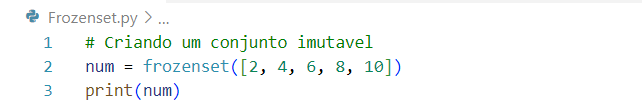
\includegraphics[width=12cm]{frozenset} 
		\newline
		Fonte: Criado por Mariana Cossetti Dalfior
	\end{center}
\end{figure}

\begin{figure}[H]
	\begin{center}
		\caption{Resultado do c\'{o}digo fonte do exemplo do uso do \textsl{frozenset}} \label{resulfrozenset}
		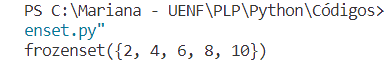
\includegraphics[width=9cm]{resulfrozenset} 
		\newline
		Fonte: Criado por Mariana Cossetti Dalfior
	\end{center}
\end{figure}
			
%%%.........................................................................................%%%
\subsection{Tipos Mapeamento}
%%%.........................................................................................%%%
Os tipo de dados de mapeamento se referem a uma cole\c{c}\~{a}o de pares chave-valor, em que os valores podem ser acessados atrav\'{e}s de suas chaves correspondentes. Os dois tipos principais de mapeamento em Python s\~{a}o:
%%%¨¨¨¨¨¨¨¨¨¨¨¨¨¨¨¨¨¨¨¨¨¨¨¨¨¨¨¨¨¨¨¨¨¨¨¨¨¨¨¨¨¨¨¨¨¨¨¨¨¨¨¨¨¨¨¨¨¨¨¨¨¨¨¨¨¨¨¨¨¨¨¨¨¨¨¨¨¨¨¨¨¨¨¨¨¨¨¨¨%%%
\subsubsection{Dicion\'{a}rios}
%%%¨¨¨¨¨¨¨¨¨¨¨¨¨¨¨¨¨¨¨¨¨¨¨¨¨¨¨¨¨¨¨¨¨¨¨¨¨¨¨¨¨¨¨¨¨¨¨¨¨¨¨¨¨¨¨¨¨¨¨¨¨¨¨¨¨¨¨¨¨¨¨¨¨¨¨¨¨¨¨¨¨¨¨¨¨¨¨¨¨%%%
Os dicion\'{a}rio em Pyhton s\~{a}o um tipo de mapeamento que possibilitam armazenar pares com valores em suas chaves correspondentes. Diferente dos valores que podem ser alterados e de qualquer tipo de dados, as chaves s\~{a}o \'{u}nicas e imut\'{a}veis. A formata\c{c}\~{a}o utilizada nos dicion\'{a}rio s\~{a}o as \textsl{'\{\}'} e os pares de chave-valor s\~{a}o separados por v\'{\i}rgulas. A seguir \'{e} poss\'{\i}vel observar o c\'{o}digo fonte \ref{fontedicionario} e o resultado \ref{resuldicionario} do exemplo da utiliza\c{c}\~{a}o de um dicion\'{a}rio em Python: \newline

\begin{lstlisting}
>>> # definindo um dicionario
>>> time_vasco = {"nome": "Capasso", "idade": 27, "posicao": 
	"zagueiro"}
>>> 
>>> # acessando valores no dicionario
>>> print(time_vasco["nome"]) 
Capasso
>>> 
>>> # atualizando valores
>>> time_vasco["nome"] = "Robson Bambu"
>>> time_vasco["idade"] = 25 
>>>
>>> # acessando valores atualizados no dicionario
>>> print(time_vasco["nome"]) 
Robson Bambu
\end{lstlisting}	

\begin{figure}[H]
	\begin{center}
		\caption{C\'{o}digo fonte do exemplo do uso de dicion\'{a}rio} \label{fontedicionario}
		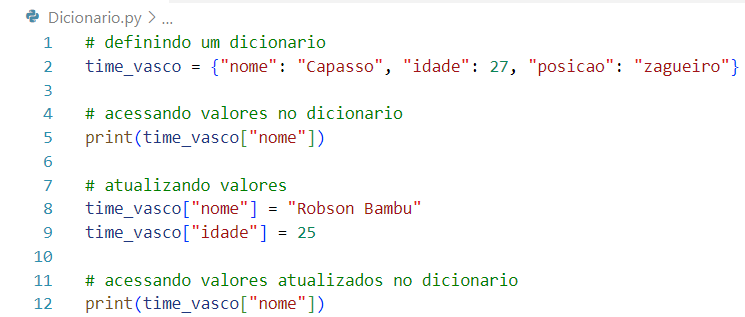
\includegraphics[width=12cm]{dicionario} 
		\newline
		Fonte: Criado por Mariana Cossetti Dalfior
	\end{center}
\end{figure}

\begin{figure}[H]
	\begin{center}
		\caption{Resultado do c\'{o}digo fonte do exemplo do uso de dicion\'{a}rio} \label{resuldicionario}
		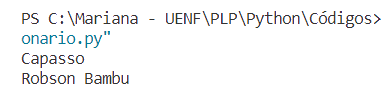
\includegraphics[width=9cm]{resuldicionario} 
		\newline
		Fonte: Criado por Mariana Cossetti Dalfior
	\end{center}
\end{figure}

Al\'{e}m de poder modificar os valores contidos nas chaves tamb\'{e}m \'{e} poss\'{\i}vel usar m\'{e}todos como \textsl{'keys()'} e \textsl{'values()'} para conseguir uma lista com todas as chaves ou valores em um dicion\'{a}rio. A seguir \'{e} poss\'{\i}vel observar o c\'{o}digo fonte \ref{fontedicionario2} e o resultado \ref{resuldicionario2} do exemplo da utiliza\c{c}\~{a}o desses m\'{e}todos:

\begin{lstlisting}
>>> # imprime uma lista de chaves
>>> print(time_vasco.keys())
>>> 
>>> # imprime uma lista de valores
>>> print(time_vasco.values()) 
dict_keys(['nome', 'idade', 'posicao'])
dict_keys(['Robson Bambu', 25, 'zagueiro'])
\end{lstlisting}	

\begin{figure}[H]
	\begin{center}
		\caption{C\'{o}digo fonte do exemplo da utiliza\c{c}\~{a}o de m\'{e}todos em dicion\'{a}rios} \label{fontedicionario2}
		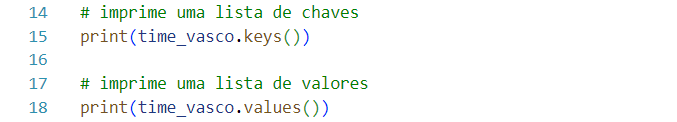
\includegraphics[width=12cm]{dicionario2} 
		\newline
		Fonte: Criado por Mariana Cossetti Dalfior
	\end{center}
\end{figure}

\begin{figure}[H]
	\begin{center}
		\caption{Resultado do c\'{o}digo fonte do exemplo da utiliza\c{c}\~{a}o de m\'{e}todos em dicion\'{a}rios} \label{resuldicionario2}
		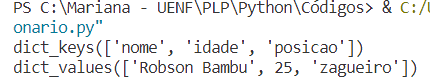
\includegraphics[width=9cm]{resuldicionario2} 
		\newline
		Fonte: Criado por Mariana Cossetti Dalfior
	\end{center}
\end{figure}

%%%¨¨¨¨¨¨¨¨¨¨¨¨¨¨¨¨¨¨¨¨¨¨¨¨¨¨¨¨¨¨¨¨¨¨¨¨¨¨¨¨¨¨¨¨¨¨¨¨¨¨¨¨¨¨¨¨¨¨¨¨¨¨¨¨¨¨¨¨¨¨¨¨¨¨¨¨¨¨¨¨¨¨¨¨¨¨¨¨¨%%%
\subsubsection{Defaultdicts}
%%%¨¨¨¨¨¨¨¨¨¨¨¨¨¨¨¨¨¨¨¨¨¨¨¨¨¨¨¨¨¨¨¨¨¨¨¨¨¨¨¨¨¨¨¨¨¨¨¨¨¨¨¨¨¨¨¨¨¨¨¨¨¨¨¨¨¨¨¨¨¨¨¨¨¨¨¨¨¨¨¨¨¨¨¨¨¨¨¨¨%%%
Os defaultdict s\~{a}o objetos parecidos com os dicion\'{a}rios, por\'{e}m possuem como diferencial a possibilidade de definir valores padr\~{a}o para chaves que n\~{a}o existem. Mesmo com isso, eles agem como um dicion\'{a}rio comum, mas quando uma chave \'{e} acessada e ela ainda n\~{a}o existe, no lugar de levantar um erro chamado {'KeyError'}, ele retorna um valor padr\~{a}o que foi definido pelo usu\'{a}rio. Esse valor \'{e} determinado na cria\c{c}\~{a}o do defaultdict. A seguir \'{e} poss\'{\i}vel observar o c\'{o}digo fonte \ref{fontedefaultdict} e o resultado \ref{resuldefaultdict} do exemplo que retornar\'{a} '\textsl{[]}' quando a chave que n\~{a}o existe for acessada:

\begin{lstlisting}
>>> #importando biblioteca
>>> from collections import defaultdict
>>>
>>> # criando um defaultdict com uma lista vazia
>>> vasco = defaultdict(list)
>>> 
>>> # adicionando valores ao defaultdict
>>> vasco['goleiro'].append('Leo Jardim')
>>> vasco['goleiro'].append('Ivan')
>>> vasco['atacante'].append('Gabriel Pec')
>>> vasco['atacante'].append('Pedro Raul')
>>>
>>> # acessando valores no defaultdict
>>> print(vasco['goleiro'])   
['Leo Jardim', 'Ivan']
>>> print(vasco['atacante'])
['Gabriel Pec', 'Pedro Raul']
>>> print(vasco['zagueiro'])
[]
\end{lstlisting}	

\begin{figure}[H]
	\begin{center}
		\caption{C\'{o}digo fonte do exemplo do uso do \textsl{defaultdict}} \label{fontedefaultdict}
		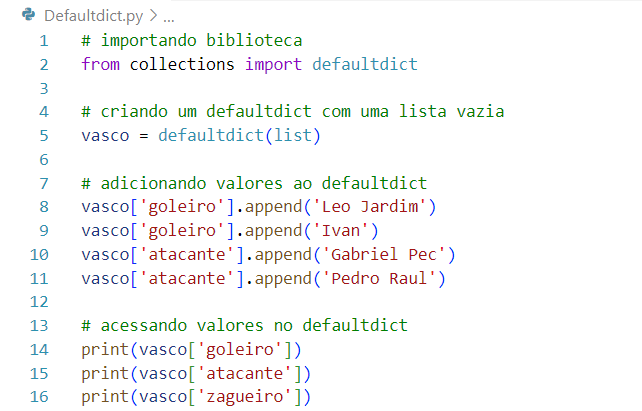
\includegraphics[width=12cm]{defaultdict} 
		\newline
		Fonte: Criado por Mariana Cossetti Dalfior
	\end{center}
\end{figure}

\begin{figure}[H]
	\begin{center}
		\caption{Resultado do c\'{o}digo fonte do exemplo do uso do \textsl{defaultdict}} \label{resuldefaultdict}
		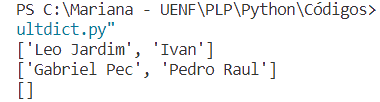
\includegraphics[width=9cm]{resuldefaultdict} 
		\newline
		Fonte: Criado por Mariana Cossetti Dalfior
	\end{center}
\end{figure}

%%%.........................................................................................%%%		
	\subsection{Metaprograma\c{c}\~{a}o de classes}
%%%.........................................................................................%%%
A metaprograma\c{c}\~{a}o de classe \'{e} a arte de criar ou customizar classes em tempo de execu\c{c}\~{a}o. As classes s\~{a}o objetos de primeira classe em Python, portanto, uma fun\c{c}\~{a}o pode ser usada para criar uma nova classe a qualquer momento, sem usar a palavra-chave \textsl{class}. Decoradores de classe tamb\'{e}m s\~{a}o fun\c{c}\~{o}es, mas projetados para inspecionar, alterar e at\'{e} mesmo substituir a classe decorada por outra classe. Finalmente, as metaclasses s\~{a}o a ferramenta mais avan\c{c}ada para a metaprograma\c{c}\~{a}o de classes: elas permitem que voc\^{e} crie categorias totalmente novas de classes com caracter\'{\i}sticas especiais.

%%%¨¨¨¨¨¨¨¨¨¨¨¨¨¨¨¨¨¨¨¨¨¨¨¨¨¨¨¨¨¨¨¨¨¨¨¨¨¨¨¨¨¨¨¨¨¨¨¨¨¨¨¨¨¨¨¨¨¨¨¨¨¨¨¨¨¨¨¨¨¨¨¨¨¨¨¨¨¨¨¨¨¨¨¨¨¨¨¨¨%%%
		\subsubsection{Decoradores de classe}
%%%¨¨¨¨¨¨¨¨¨¨¨¨¨¨¨¨¨¨¨¨¨¨¨¨¨¨¨¨¨¨¨¨¨¨¨¨¨¨¨¨¨¨¨¨¨¨¨¨¨¨¨¨¨¨¨¨¨¨¨¨¨¨¨¨¨¨¨¨¨¨¨¨¨¨¨¨¨¨¨¨¨¨¨¨¨¨¨¨¨%%%

Um decorador de classe \'{e} um recurso de chamada que se comporta de forma semelhante a um decorador de fun\c{c}\~{a}o: ele obt\'{e}m a classe decorada como argumento e deve retornar uma classe para substituir a classe decorada. Os decoradores de classe geralmente retornam a pr\'{o}pria classe decorada, depois de injetar mais m\'{e}todos nela por meio da atribui\c{c}\~{a}o de atributos. Provavelmente, a raz\~{a}o mais comum para escolher um decorador de classe em vez do simples \textsl{\_\_init\_subclass\_\_} \'{e} evitar a interfer\^{e}ncia com outros recursos de classe, como heran\c{c}a e metaclasses. A seguir \'{e} poss\'{\i}vel observar o c\'{o}digo fonte \ref{fontedecoradores} e o resultado \ref{resuldecoradores} do exemplo de decoradores:

\begin{lstlisting}
>>> @checked
>>> @dataclass
>>> class Filme:
>>> 	titulo: str
>>> 	ano: int
>>> 	preco: float
>>>
>>> filme = Filme(titulo= 'O Poderoso Chefao', ano= 1972, preco= 137.6)
>>> 
>>> print(filme.titulo) 
O Poderoso Chefao
>>> print(filme)
Filme(titulo= 'O Poderoso Chefao', ano= 1972, preco= 137.6)
\end{lstlisting}

\begin{figure}[H]
	\begin{center}
		\caption{C\'{o}digo fonte do exemplo do uso de decoradores de classe} \label{fontedecoradores}
		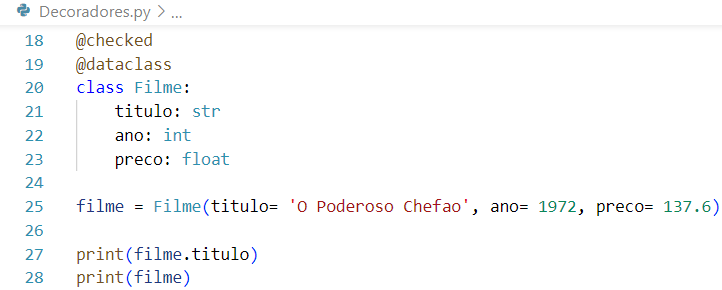
\includegraphics[width=12cm]{decoradores} 
		\newline
		Fonte: Criado por Mariana Cossetti Dalfior
	\end{center}
\end{figure}

\begin{figure}[H]
	\begin{center}
		\caption{Resultado do c\'{o}digo fonte do exemplo do uso de decoradores de classe} \label{resuldecoradores}
		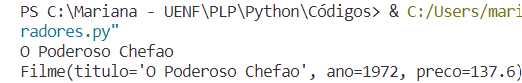
\includegraphics[width=9cm]{resuldecoradores} 
		\newline
		Fonte: Criado por Mariana Cossetti Dalfior
	\end{center}
\end{figure}

%%%¨¨¨¨¨¨¨¨¨¨¨¨¨¨¨¨¨¨¨¨¨¨¨¨¨¨¨¨¨¨¨¨¨¨¨¨¨¨¨¨¨¨¨¨¨¨¨¨¨¨¨¨¨¨¨¨¨¨¨¨¨¨¨¨¨¨¨¨¨¨¨¨¨¨¨¨¨¨¨¨¨¨¨¨¨¨¨¨¨%%%
		\subsubsection{Metaclasses}
%%%¨¨¨¨¨¨¨¨¨¨¨¨¨¨¨¨¨¨¨¨¨¨¨¨¨¨¨¨¨¨¨¨¨¨¨¨¨¨¨¨¨¨¨¨¨¨¨¨¨¨¨¨¨¨¨¨¨¨¨¨¨¨¨¨¨¨¨¨¨¨¨¨¨¨¨¨¨¨¨¨¨¨¨¨¨¨¨¨¨%%%

A classe de tipo \'{e} uma metaclasse: uma classe que constr\'{o}i classes. Em outras palavras, as inst\^{a}ncias da classe de tipo s\~{a}o classes. A biblioteca padr\~{a}o fornece algumas outras metaclasses, mas \textsl{type} \'{e} a padr\~{a}o. A seguir \'{e} poss\'{\i}vel observar o c\'{o}digo fonte \ref{fontemetaclasse} e o resultado \ref{resulmetaclasse} desse exemplo:

\begin{lstlisting}
>>> print(type(7))
<class 'int'>
>>> print(type(int))
<class 'type'>
>>>	  
\end{lstlisting}

\begin{figure}[H]
	\begin{center}
		\caption{C\'{o}digo fonte do exemplo do uso de metaclasse} \label{fontemetaclasse}
		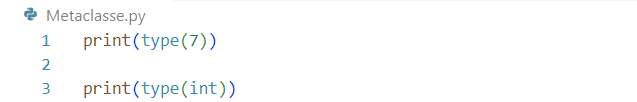
\includegraphics[width=12cm]{metaclasse} 
		\newline
		Fonte: Criado por Mariana Cossetti Dalfior
	\end{center}
\end{figure}

\begin{figure}[H]
	\begin{center}
		\caption{Resultado do c\'{o}digo fonte do exemplo do uso de metaclasse} \label{resulmetaclasse}
		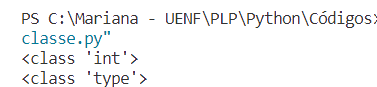
\includegraphics[width=9cm]{resulmetaclasse} 
		\newline
		Fonte: Criado por Mariana Cossetti Dalfior
	\end{center}
\end{figure}

%%%.........................................................................................%%%
	\subsection{Heran\c{c}as}
%%%.........................................................................................%%%

A heran\c{c}a \'{e} um mecanismo da programa\c{c}\~{a}o orientada a objetos que visa facilitar a reutiliza\c{c}\~{a}o de c\'{o}digo. A ideia fundamental \'{e} que as classes possam ser organizadas em uma hierarquia, onde as novas classes podem herdar os m\'{e}todos e propriedades das classes existentes (que podem ter sido herdadas de outras classes anteriores) e, ao mesmo tempo, adicionar seus pr\'{o}prios m\'{e}todos e propriedades.

%%%¨¨¨¨¨¨¨¨¨¨¨¨¨¨¨¨¨¨¨¨¨¨¨¨¨¨¨¨¨¨¨¨¨¨¨¨¨¨¨¨¨¨¨¨¨¨¨¨¨¨¨¨¨¨¨¨¨¨¨¨¨¨¨¨¨¨¨¨¨¨¨¨¨¨¨¨¨¨¨¨¨¨¨¨¨¨¨¨¨%%%
		\subsubsection{Heran\c{c}a Simples}
%%%¨¨¨¨¨¨¨¨¨¨¨¨¨¨¨¨¨¨¨¨¨¨¨¨¨¨¨¨¨¨¨¨¨¨¨¨¨¨¨¨¨¨¨¨¨¨¨¨¨¨¨¨¨¨¨¨¨¨¨¨¨¨¨¨¨¨¨¨¨¨¨¨¨¨¨¨¨¨¨¨¨¨¨¨¨¨¨¨¨%%%
Na heran\c{c}a, \'{e} comum utilizar a chamada "heran\c{c}a simples", em que as novas classes s\~{a}o derivadas das classes existentes. \'{E} poss\'{\i}vel criar m\'{u}ltiplas classes derivadas, formando uma hierarquia de classes. Na busca por m\'{e}todos e propriedades, a procura ocorre de baixo para cima na hierarquia, de forma similar \`{a} busca em \textsl{namespaces} locais e globais. A seguir \'{e} poss\'{\i}vel observar o c\'{o}digo fonte \ref{fonteherancasimples} e o resultado \ref{resulherancasimples} do exemplo de heran\c{c}a simples:
			
\begin{lstlisting}
>>> class Pendrive(object):
>>> def __init__(self, tamanho, interface='2.0'):
>>> self.tamanho = tamanho
>>> self.interface = interface
>>> 
>>> class MP3Player(Pendrive):
>>> def __init__(self, tamanho, interface='2.0', turner=False):
>>> super().__init__(tamanho, interface)
>>> self.turner = turner
>>>
>>> mp3 = MP3Player(1024)
>>> print('%s\n%s\n%s' % (mp3.tamanho, mp3.interface, mp3.turner))
1024
2.0
False
\end{lstlisting}

\begin{figure}[H]
	\begin{center}
		\caption{C\'{o}digo fonte do exemplo do uso de heran\c{c}a simples} \label{fonteherancasimples}
		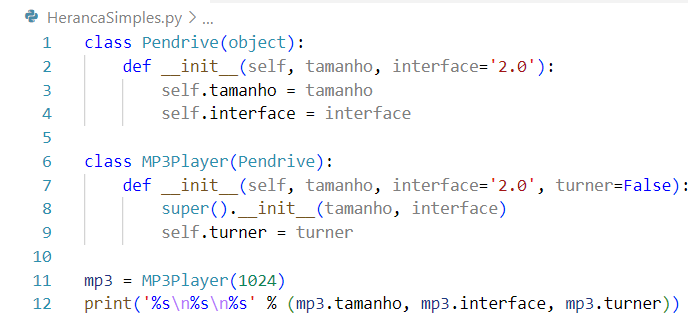
\includegraphics[width=12cm]{herancasimples} 
		\newline
		Fonte: Criado por Mariana Cossetti Dalfior
	\end{center}
\end{figure}

\begin{figure}[H]
	\begin{center}
		\caption{Resultado do c\'{o}digo fonte do exemplo do uso de heran\c{c}a simples} \label{resulherancasimples}
		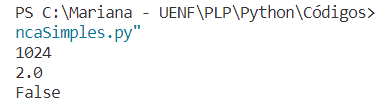
\includegraphics[width=9cm]{resulherancasimples} 
		\newline
		Fonte: Criado por Mariana Cossetti Dalfior
	\end{center}
\end{figure}

Essa abordagem permite que as classes filhas herdem o comportamento e as caracter\'{\i}sticas das classes pai, enquanto t\^{e}m a flexibilidade de adicionar ou modificar essas caracter\'{\i}sticas conforme necess\'{a}rio, dentro da nova classe. A heran\c{c}a, portanto, promove a reutiliza\c{c}\~{a}o de c\'{o}digo ao facilitar o aproveitamento de implementa\c{c}\~{o}es existentes e a cria\c{c}\~{a}o de classes especializadas com base nessas implementa\c{c}\~{o}es.

%%%¨¨¨¨¨¨¨¨¨¨¨¨¨¨¨¨¨¨¨¨¨¨¨¨¨¨¨¨¨¨¨¨¨¨¨¨¨¨¨¨¨¨¨¨¨¨¨¨¨¨¨¨¨¨¨¨¨¨¨¨¨¨¨¨¨¨¨¨¨¨¨¨¨¨¨¨¨¨¨¨¨¨¨¨¨¨¨¨¨%%%	
		\subsubsection{Heran\c{c}as M\'{u}ltiplas}
%%%¨¨¨¨¨¨¨¨¨¨¨¨¨¨¨¨¨¨¨¨¨¨¨¨¨¨¨¨¨¨¨¨¨¨¨¨¨¨¨¨¨¨¨¨¨¨¨¨¨¨¨¨¨¨¨¨¨¨¨¨¨¨¨¨¨¨¨¨¨¨¨¨¨¨¨¨¨¨¨¨¨¨¨¨¨¨¨¨¨%%%
A heran\c{c}a m\'{u}ltipla permite que uma nova classe seja derivada de duas ou mais classes existentes ao mesmo tempo. A seguir \'{e} poss\'{\i}vel observar o c\'{o}digo fonte \ref{fonteherancamultipla} e o resultado \ref{resulherancamultipla} do exemplo de heran\c{c}a m\'{u}ltipla:

\begin{lstlisting}
>>> class Terrestre(object):
>>> 	se_move_em_terra = True
>>>
>>> 	def __init__(self, velocidade=100):
>>> 		self.velocidade_em_terra = velocidade
>>> 
>>> class Aquatico(object):
>>> 	se_move_na_agua = True
>>>
>>> 	def __init__(self, velocidade=5):
>>> 		self.velocidade_agua = velocidade
>>>
>>> class Carro(Terrestre):
>>> 	rodas = 4
>>>
>>> 	def __init__(self, velocidade=120, pistoes=4):
>>> 		self.pistoes = pistoes
>>> 		super().__init__(velocidade=velocidade)
>>>
>>> class Barco(Aquatico):
>>>
>>> 	def __init__(self, velocidade=6, helices=1):
>>> 		self.helices = helices
>>> 		super().__init__(velocidade=velocidade)
>>> 
>>> class Anfibio(Carro, Barco):
>>> 
>>>     def __init__(self, velocidade_em_terra=80, 
                    velocidade_na_agua=4, pistoes=6, helices=2):
>>> 		Carro.__init__(self, velocidade=velocidade_em_terra, 
				pistoes=pistoes)
>>> 		Barco.__init__(self, velocidade=velocidade_na_agua, 
				helices=helices)
>>>
>>> novo_anfibio = Anfibio()
>>> for atr in dir(novo_anfibio):
>>> 	if not atr.startswith('__'):
>>> 		print(atr, '=', getattr(novo_anfibio, atr))
helices = 2
pistoes = 6
rodas = 4
se_move_em_terra = True
se_move_em_agua = True
velocidade_agua = 4
velocidade_terra = 80
\end{lstlisting}

\begin{figure}[H]
	\begin{center}
		\caption{C\'{o}digo fonte do exemplo do uso de heran\c{c}a m\'{u}ltipla} \label{fonteherancamultipla}
		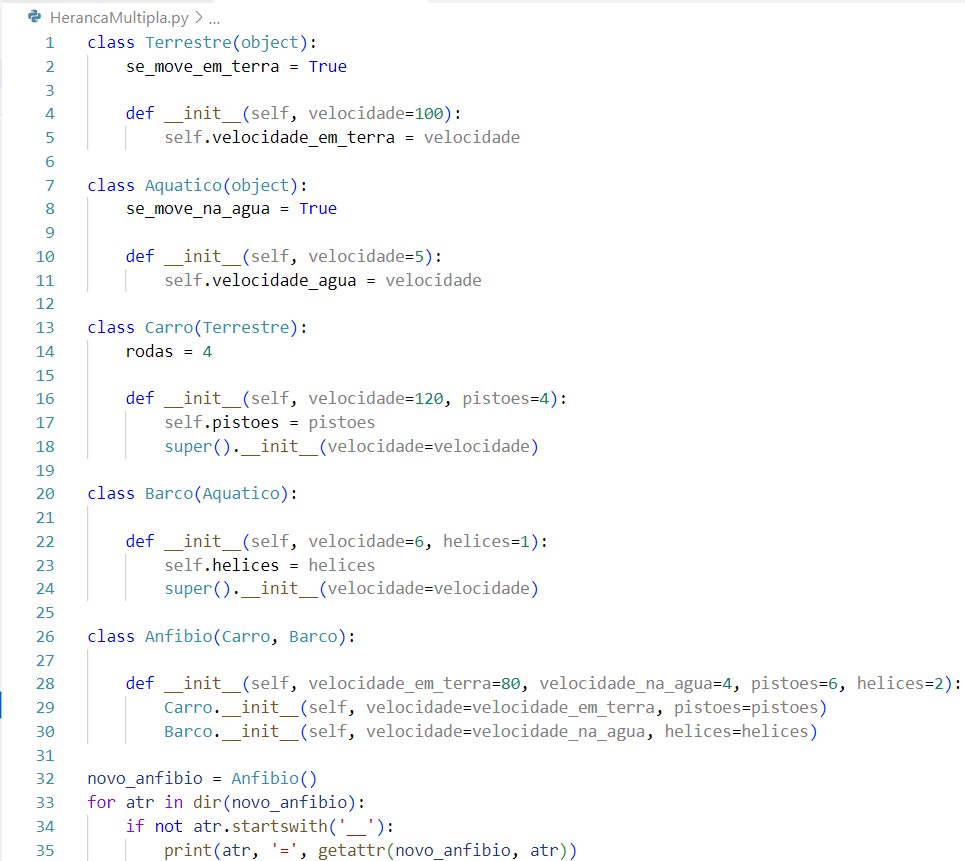
\includegraphics[width=12cm]{herancamultipla} 
		\newline
		Fonte: Criado por Mariana Cossetti Dalfior
	\end{center}
\end{figure}

\begin{figure}[H]
	\begin{center}
		\caption{Resultado do c\'{o}digo fonte do exemplo do uso de heran\c{c}a m\'{u}ltipla} \label{resulherancamultipla}
		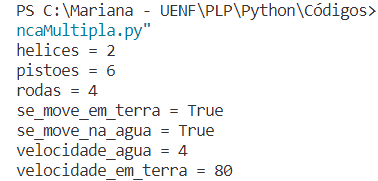
\includegraphics[width=9cm]{resulherancamultipla} 
		\newline
		Fonte: Criado por Mariana Cossetti Dalfior
	\end{center}
\end{figure}

A diferen\c{c}a mais not\'{a}vel em rela\c{c}\~{a}o \`{a} heran\c{c}a simples est\'{a} na ordem de resolu\c{c}\~{a}o de m\'{e}todos (MRO, do ingl\^{e}s Method Resolution Order). A heran\c{c}a m\'{u}ltipla \'{e} um recurso controverso devido \`{a} sua complexidade, podendo tornar o design do c\'{o}digo confuso e menos claro.

%%%=========================================================================================%%%
\section{Fun\c{c}\~{o}es Geradoras}
%%%=========================================================================================%%%

Segundo \cite{Sarma2021}, a \'{u}nica sintaxe que distingue uma fun\c{c}\~{a}o simples de uma geradora \'{e} o fato de que a \'{u}ltima possui uma palavra-chave \textsl{yield} em algum lugar de seu corpo. Qualquer fun\c{c}\~{a}o Python que tenha essa palavra-chave em seu corpo \'{e} uma fun\c{c}\~{a}o geradora: uma fun\c{c}\~{a}o que, quando chamada, retorna um objeto gerador. Em outras palavras, uma fun\c{c}\~{a}o de geradora \'{e} uma f\'{a}brica de geradores. A seguir \'{e} poss\'{\i}vel observar o c\'{o}digo fonte \ref{fonteherancamultipla} e o resultado \ref{resulherancamultipla} do exemplo utilizando fun\c{c}\~{a}o geradora:

\begin{lstlisting}
>>> # Funcao geradora que produz tres numeros
>>> def gen_123():
>>>	  yield 1
>>>	  yield 2
>>>	  yield 3
>>>
>>> for i in gen_123():
>>>	print(i)
1
2
3
\end{lstlisting}

\begin{figure}[H]
	\begin{center}
		\caption{C\'{o}digo fonte do exemplo do uso de fun\c{c}\~{o}es geradoras} \label{fontefuncaogeradora}
		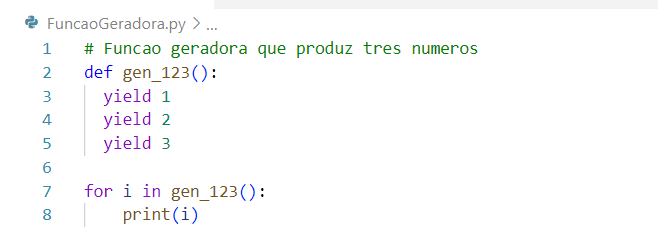
\includegraphics[width=12cm]{funcaogeradora} 
		\newline
		Fonte: Criado por Mariana Cossetti Dalfior
	\end{center}
\end{figure}

\begin{figure}[H]
	\begin{center}
		\caption{Resultado do c\'{o}digo fonte do exemplo do uso de fun\c{c}\~{o}es geradoras} \label{resulfuncaogeradora}
		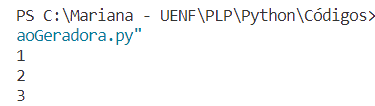
\includegraphics[width=9cm]{resulfuncaogeradora} 
		\newline
		Fonte: Criado por Mariana Cossetti Dalfior
	\end{center}
\end{figure}

Dessa forma, foi criada uma fun\c{c}\~{a}o geradora \textsl{gen\_123()} e para ela foram criadas tr\^{e}s instru\c{c}\~{o}es \textsl{yield} para retornar os valores 1, 2 e 3, respectivamente. Depois foi criado um loop com o \textsl{for} para que esses n\'{u}meros fossem mostrados, atrav\'{e}s do \textsl{print(i)}.
